\documentclass[12pt,a4paper,hidelinks]{article}
\usepackage{amsmath}
\usepackage{amsfonts}
\usepackage{amssymb}
\usepackage{makeidx}
\usepackage[left=2cm,right=2cm,top=2cm,bottom=2cm]{geometry}
\usepackage{parskip}
\usepackage{hyperref}
\usepackage{graphicx}

\usepackage{algorithm,algpseudocode}

\usepackage{listings}
\lstset{
	breaklines=true,
	tabsize=4,
	numbers=left
}

\def\algorithmautorefname{Algorithm}

\author{Bert Peters --- s1147919}
\title{Social Network Analysis for Computer Scientists --- Assignment 1}
\begin{document}

\maketitle

\section{Neighbourhoods}

\begin{enumerate}
	\item This is true only for a complete graph, because for this to happen every node should be connected to every other node.
	
	\item This computes the centrality, with a lower number meaning a more central node.
	
	\item To define the reverse $k$ neighbourhood, we first define the reverse neighbourhood as follows:
	$$
		N'(W) = \{ w \in V : v \in W \land (v, w) \in E \}
	$$
	
	Then, after defining that, we modify that to use a $k$ reversed neighbourhood an define the following:
	\begin{align*}
		N_0'(W) & = W \\
		N_k'(W) & = N'(N_{k - 1}'(W) \cup N_{k - 1}'(W)
	\end{align*}
	
	\item Two nodes $v$ and $w$ are part of the same strongly connected component iff
	$$
		N_k(\{v\}) \cap N'_k(\{v\}) = N_k(\{w\}) \cap N'_k(\{w\})
	$$
	
	for some $k \geq 0$.
	
	\item The algorithm shown in \autoref{algo:components} shows how this could be done using the $N_k(W)$ method. After the algorithm is done, $n$ contains the number of components.
\end{enumerate}

\begin{algorithm}
\caption{Computing the number of connected components in an undirected network.}
\label{algo:components}

\begin{algorithmic}
	\State $n \gets 0$
	\While{$V \neq \emptyset$}
		\State Pick a random $v \in V$
		\State $p \gets 0$
		\While{$|N_{p + 1}(\{v\})| > |N_p(\{v\})|$}
			\State $p \gets p + 1$
		\EndWhile
		
		\State $n \gets n + 1$
		\State $V \gets V \setminus N_p(\{v\})$
	\EndWhile
\end{algorithmic}

\end{algorithm}

\section{Diameter computation}

I execute the BoundingDiameters\footnote{F.W. Takes and W.A. Kosters, Determining the Diameter of Small World Networks, in \textit{Proceedings of the 20th ACM International Conference on Information
and Knowledge Management} (CIKM), pp. 1191-1196, 2011} on the graph provided on paper. As this is rather complex to shown in \LaTeX, I illustrate the actions I perform in text.

\begin{enumerate}
	\item We start with selecting an initial node with the lowest lower bound. As there are no known bounds, we select the node with the highest degree. This is node $F$, as it has degree 6. The longest shortest path is from $F \rightarrow T$, of length 5. This produces the bounds as shown in \autoref{tab:it1}.
	
		\begin{table}
			\centering
			\begin{tabular}{l | r | r}
				Node & $\varepsilon_L$ & $\varepsilon_U$ \\
				\hline
				$A$ & 5 & 7 \\
				$B$ & 5 & 7 \\
				$C$ & 5 & 6 \\
				$D$ & 5 & 6 \\
				$E$ & 5 & 6 \\
				$F$ & 5 & 5 \\
				$G$ & 5 & 7 \\
				$H$ & 5 & 6 \\
				$I$ & 5 & 8 \\
				$J$ & 5 & 6 \\
				$K$ & 5 & 7 \\
				$L$ & 5 & 6 \\
				$M$ & 5 & 7 \\
				$N$ & 5 & 7 \\
				$P$ & 5 & 7 \\
				$Q$ & 5 & 8 \\
				$R$ & 5 & 8 \\
				$S$ & 5 & 9 \\
				$T$ & 5 & 10 \\
			\end{tabular}
			\caption{Eccentricity bounds after 1 iteration of the algorithm.}
			\label{tab:it1}
		\end{table}
	
	\item After this, we already have some interesting bounds.  Because we technically did select the lowest lower bound, we select the highest upper bound this time. This is node $T$, with an upper bound of 10. The longest path is $T \rightarrow I$, of length 8. After recomputing the bounds, we arrive at the bounds as shown in \autoref{tab:it2}.
	
		\begin{table}
			\centering
			\begin{tabular}{l | r | r}
				Node & $\varepsilon_L$ & $\varepsilon_U$ \\
				\hline
				$A$ & 7 & 7 \\
				$B$ & 7 & 7 \\
				$C$ & 6 & 6 \\
				$D$ & 6 & 6 \\
				$E$ & 6 & 6 \\
				$F$ & 5 & 5 \\
				$G$ & 7 & 7 \\
				$H$ & 6 & 6 \\
				$I$ & 8 & 8 \\
				$J$ & 6 & 6 \\
				$K$ & 7 & 7 \\
				$L$ & 5 & 6 \\
				$M$ & 5 & 7 \\
				$N$ & 5 & 7 \\
				$P$ & 5 & 7 \\
				$Q$ & 5 & 8 \\
				$R$ & 5 & 8 \\
				$S$ & 7 & 9 \\
				$T$ & 8 & 8 \\
			\end{tabular}
			\caption{Eccentricity bounds after 2 iteration of the algorithm.}
			\label{tab:it2}
		\end{table}
	
	\item Now, most bounds are already tight, and there is one single node that can still contribute to the diameter, node $S$, because it is the only node with an upper bound larger than 8. Intuitively, you can see that it will not, because all paths from $T$ go through $S$, but we are technically not done yet. Computing the actual eccentricity, we know it actually is 7, and that the diameter of the network is 8.
\end{enumerate}

The naive method would need to do a breadth first search starting from every node. As shown above, I have only done three.

\section{An Online Social Network}

\subsection{Number of edges}

As the file contains one link per line, the number of links can be determined by counting the number of lines. This does not require a program, but can be done with a little snippet of bash.

\lstinputlisting[language=bash]{edges.sh}

Or, rather, just use the \texttt{wc} utility. The results for this exercise are incorporated in \autoref{tab:counts}.

\subsection{Number of nodes}

Like for the previous exercise, a full fledged parser is still not necessary. Instead, I combine the two columns using \texttt{awk}, \texttt{sort} them, take unique rows, and finally count lines again. The exact code is shown in Listing \ref{script:nodes} and the results can be found in \autoref{tab:counts}.

\lstinputlisting[
	language=bash,
	caption=Node counter script.,
	label=script:nodes,
	float
]{nodes.sh}

The parameters for sort are slightly unusual. We do this to improve performance, so that this script can handle the \texttt{huge.in} network. The compress program allows us to use less disk space for temporaries, which is neccessary to prevent disk space issues, and we increase the buffer size to improve overall performance.

\begin{table}
\centering
\begin{tabular}{l | r | r | l | r}
Filename & {\centering $|E|$} & $|V|$ & Directed & Largest component\\
\hline
medium.in & 16631 & 2426 & Possibly & 2000 \\
large.in & 14855842 & 456626 & Yes & 456290 \\
huge.in & 892263106 & 8113017 & Yes & 8083964
\end{tabular}
\caption{Various counts for the network files}
\label{tab:counts}
\end{table}

\subsection{Degree distribution}

To compute the in or out degree for a node, we can simply count the number of times that a number occurs in the source or destination column. The code for this is shown in Listing \ref{script:degrees}.

\lstinputlisting[
	language=bash,
	caption=Script for computing the degree for all nodes.,
	label=script:degrees,
	float
]{degree.sh}

After we have computed the degree for various nodes, we can use this output to make a visualisation.



\begin{figure}
	\centering
	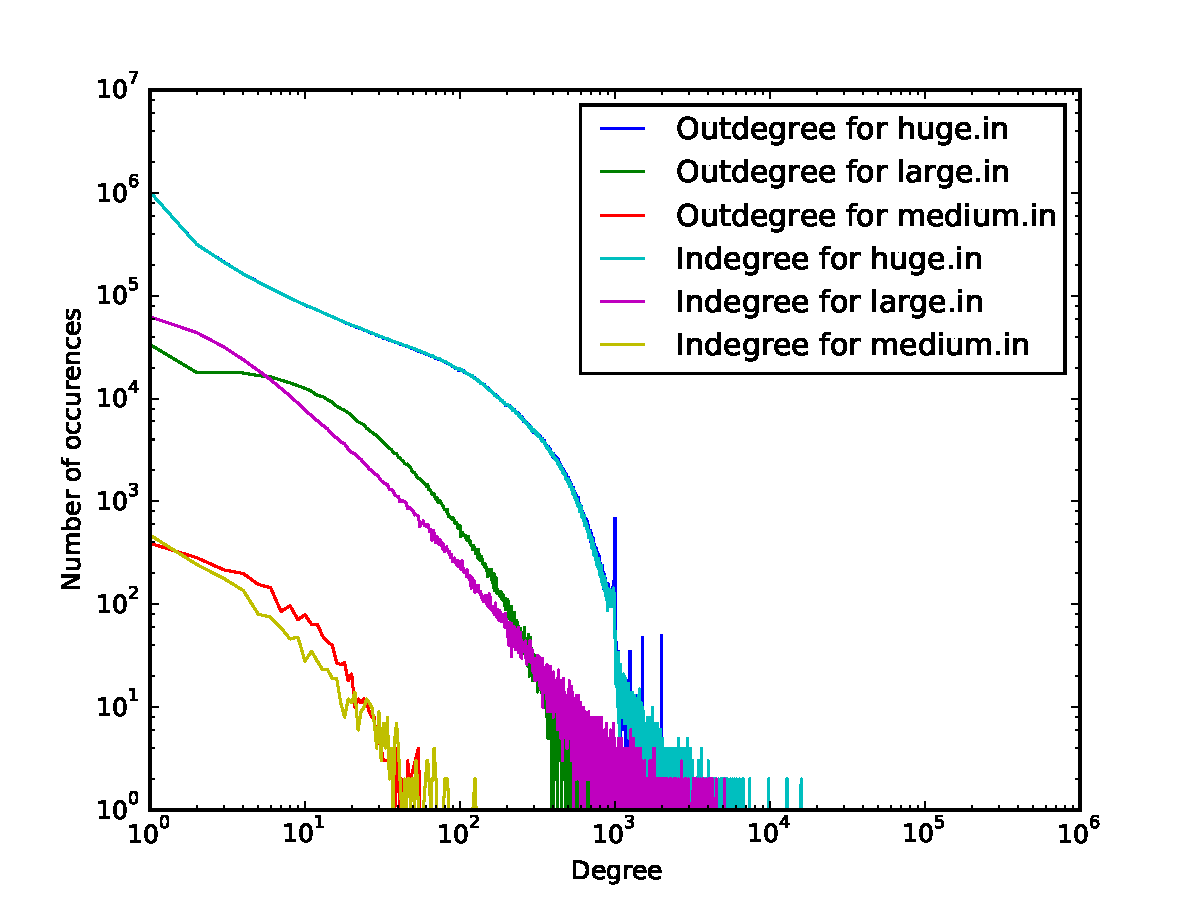
\includegraphics[scale=0.83]{degree-distributions}
	\caption{The degree distributions for all input files.}
	\label{fig:degrees}
\end{figure}

\subsection{Directedness}

To answer this question, we must agree upon the interpretation of the file. There are some cases which can lead us to an interpretation. The following statements determine this.

\begin{align}
\label{eq:somereflex} \exists u, v &: (u, v) \in E \land (v, u) \in E \\
\label{eq:allreflex} \forall u, v &: (u, v) \in E \implies (v, u) \in E \\
\label{eq:noreflex}\nexists u, v &: (u, v) \in E \land (v, u) \in E
\end{align}

If \ref{eq:allreflex} holds, we are clearly in an undirected graph, because every edge is reflexive.

If \ref{eq:somereflex} and holds and \ref{eq:allreflex} does not, we are clearly in a directed graph because there are some reflexive connections, but not all of them are.

If, however, \ref{eq:noreflex} holds, there are no reflexive edges. This means that we can interpret the graph as either undirected or directed, because we can interpret each edge as also going back.

Once again, we implement this in bash, as it is very simple. We use \texttt{awk} to put any edge listing $(u, v)$ in the file in asceding order, so that when we sort the file, edges and returning edges are next to each other. This allows us to remove duplicates, and then analyze the number of lines that remain. We can differentiate these counts in two categories.

\begin{align*}
2 \times & |E_{unique}| = |E| & \implies & \text{Network is undirected.} \\
|E| < 2 \times & |E_{unique}| < 2 \times |E| & \implies & \text{Network is directed} \\
& |E_{unique}| = |E| & \implies & \text{Network is possibly directed}
\end{align*}

The bash script in Listing \ref{script:directed} computes $|E|$ and $|E_{unique}|$ and prints out the category the network falls in.

\lstinputlisting[
	language=bash,
	caption=Code that computes whether or not a graph is directed,
	label=script:directed,
	float
]{directed.sh}

\subsection{Largest connected component}

For this section, we consider the largest connected component to be the largest weakly connected component. This helps us, because this removes the distinction between directed and undirected networks.

To compute the largest connected component, I could not come up with a \texttt{bash}-based solution, so I reverted to using \texttt{C++}.

The algorithm works as follows. First, we store our edges into a large edge array and sort them on $u, v$. After that, we attempt to make a coloring for each node. In this coloring, connected nodes are the same color. Finally, we determine the number of occurences for the most frequent color. This is our answer. The code for this algorithm can be found in \autoref{appendix:components}.

\subsubsection*{Coloring algorithm}

The coloring algorithm is more or less a breadth first search, as described in \autoref{algo:coloring}. We know that the complexity of a breadth first search is $O(|E|)$,\footnote{Technically, this is $|V|)$, but because we consider sparse networks, $|E| \approx |V|$ so we ignore $|E|$. This simplifies our formulae.} without accounting for the complexity of determining neighbours for nodes. Because we sorted our list of edges, we can access the neighbours of $u$ using binary search in $O(B + \log |E|)$, with $B$ the number of neighbours.

In the inner loop of our algorithm, the most complex task we potentially do, is recoloring all the nodes. The way we do this is enumerating all nodes and replacing the colors we have to. This is an $O(|V|)$ operation. This happens each time we find a new directed route into an existing component. However, this rarely happens. Most of the time, we find a connected component once, because the networks are very reflexive.

So, to summarize, our theorethical complexity is $O(|V|(\log |E| + |V|))$.\footnote{We ignore the $B$ in the complexity for accessing neighbours, because the rest of the loop gets executed just as often. Therefore, it is already part of the BFS complexity.} This works out to $O(|V|^2 + |V|\log|E|) \approx O(|V|^2)$. This complexity however includes the recoloring cost, so while it is the worst case, the average case is better, and runs in $O(|V| \log |E|)$.

\begin{algorithm}
\caption{Node coloring algorithm}
\label{algo:coloring}
\begin{algorithmic}

\ForAll{$u \in V$}
	\State initialize $color_u$ as 0
\EndFor
\\
\ForAll{$u \in V$}
	\If{$color_u = 0$}
		\State $todo \gets \{u\}$
		\While{$todo \neq \emptyset$}
			\State Pick a $v$ from $todo$
			\State $todo \gets todo \setminus \{v\}$
			\If{$color_v \neq u$}
				\If{$color_v = 0$}
					\State $color_v \gets u$
					\State Add all $w : w \in N_1(v) \land  color_w \neq u$ to $todo$.
				\Else
					\State Recolor all $w : color_w = color_v$ to $u$.
				\EndIf
			\EndIf
		\EndWhile
	\EndIf
\EndFor

\end{algorithmic}
\end{algorithm}

\subsection{Visualization}

To visualize \texttt{medium.in}, I used Gephi. I chose to interpret the network as an undirected network and to visualise only the largest connected component. That component contains over 80\% of the nodes in the network, and the remaining components are very small.\footnote{Most of the components are less than 10 nodes in size.}

Coloring of nodes is done using community detection, and sizing was done by degree. The nodes were grouped using the YifanHu Multilevel algorithm, with the default parameters, and manually making it slightly more compact. I decided not to show the links, as it is mostly a clustered mess. The groupings are visible this way, and it looks nicer.

Shown in \autoref{fig:visualisation} is the final visualisation. To me, it looks something like Australia, except with way too many people in the Outback.

\begin{figure}
	\centering
	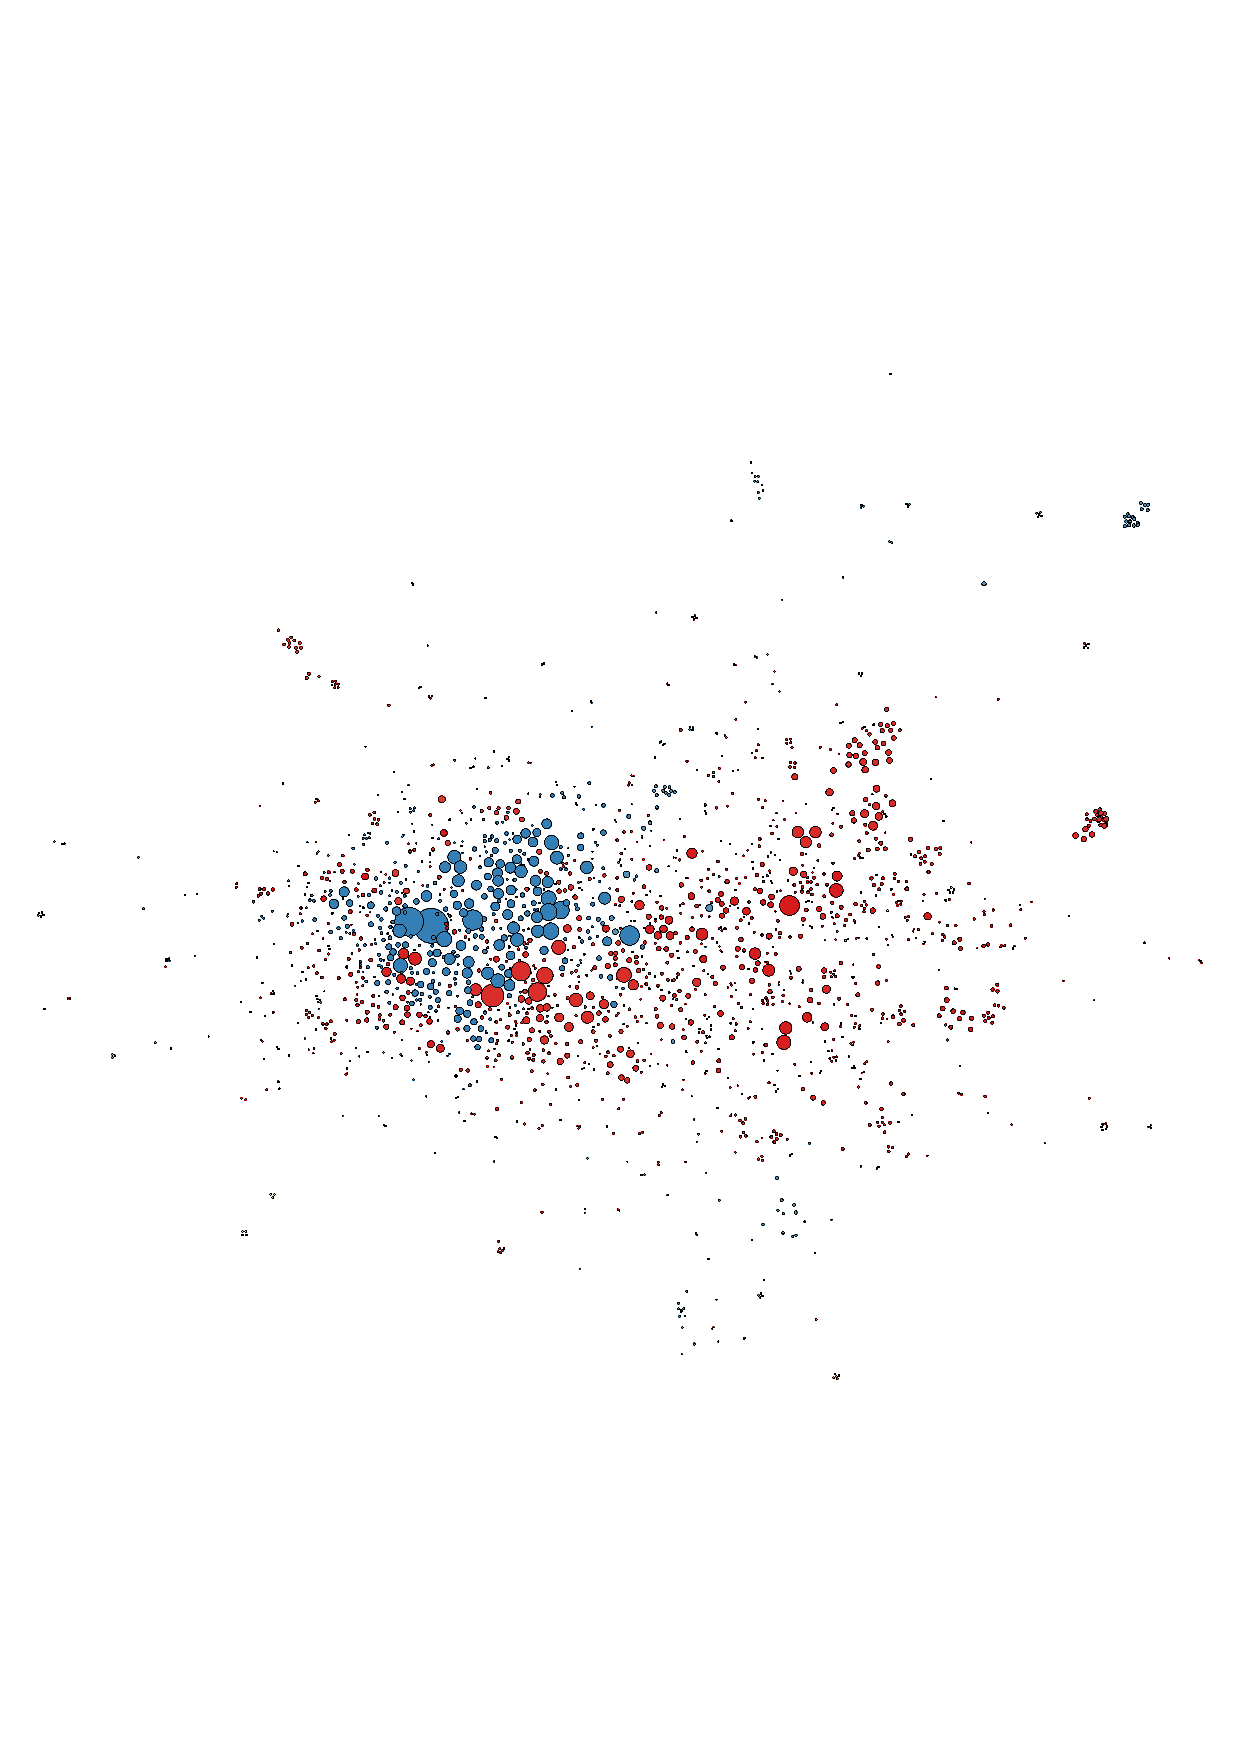
\includegraphics[scale=0.55]{visualisation}
	\caption{\texttt{medium.in} visualized}
	\label{fig:visualisation}
\end{figure}

\subsection{Analyzing \texttt{huge.in}}

Analyzing the \texttt{huge.in} network required some memory management, to store all nodes in memory. Fortunately, the Linux shell tools \texttt{awk}, \texttt{wc}, \texttt{sort}, \texttt{gzip}, and \texttt{uniq} all require very little memory, so those programs worked just as well for the \texttt{huge.in} network as it did for the others.

Moreover, the most expensive operation being done in each of the bash script files, is sorting, which requires at most $O(|E| \log |E|)$ time and $O(|E|)$ disk storage. The disk storage requirement is then reduced using \texttt{gzip}, so the actual storage requirement is significantly less.\footnote{\texttt{sort} stores sorted chunks on disk. Sorted lists of numbers happen to contain a lot of repeating strings, so in some cases, \texttt{gzip} was able to reduce the files by up to 99\%.}

The only computationally heavy exercise left is computing the largest weakly connected component. The program uses two \texttt{int}s per edge, or 8 bytes. This means 6.6 GiB for the edges alone. Furthermore, a bit of memory is allocated to store what component a node is in, but that is neglegible. My initial program used a \texttt{std::queue} for the bread first search queue. Peaking at 3.5 GiB of storage (of \texttt{int}s representing nodes), this turned out to a bit much. Instead, I used \texttt{std::set} as a todo list, forcing only a single entry per node. This has some downsides, mostly being performance and using more memory per entry. It did actually help to brng the todo-list down to 1.5 GiB of memory, allowing the program to run on a machine with at least 8.1 GiB of memory, while only doubling the execution time.

The memory footprint can still be significantly improved. The memory usage for the edges can be slimmed down to $4 \times |E| + 8 \times |V|$ by using using two arrays. One storing the destinations for edges, and one storing for each node the number of edges it has, and its starting point in the first array. Even this can be slightly slimmed down to $4 \times |E| + 4 \times |V|$ by not storing the starting point, but instead inferring it from the number of nodes already passed.\footnote{Credits to Koen \textellipsis for suggesting I do this.} I did not implement such a strategy, as it complicates reading the files, requiring either pre-sorting the input or lots of relocations while reading.

\appendix

\section{Source listing for analyze.py}

\label{appendix:analyze}

Below is the source code for \texttt{analyze.py}. The code runs with Python 2.7 and requires matplotlib.

\lstinputlisting[
	language=python
]{analyze.py}

\section{Source listing for component.cpp}

\label{appendix:components}

Below is the source for \texttt{component.cpp}. The program was compiled using the makefile in \autoref{appendix:makefile}.

\lstinputlisting[language=c++]{component.cpp}

\section{Makefile}

\label{appendix:makefile}

\lstinputlisting[
	language={[gnu]make}
]{Makefile}

\end{document}
